%%%%%%%%%%%%%%%%%%%%%%%%%%%%%%%%%%%%%%%%%%%%%%%%%%%%%%%%%%%%%%%%%%%%%%%%%%%%%%%%%%%%%%%%%%%%%%%%%%%%%%%%%%%%%%%%%%%%%%%%%%%%%%%%%%%%%%%%%%%%%%%%%%%%%%%%%%%%%%%%%%%
% Written By Michael Brodskiy
% Class: Fundamentals of Linear Systems
% Professor: I. Salama
%%%%%%%%%%%%%%%%%%%%%%%%%%%%%%%%%%%%%%%%%%%%%%%%%%%%%%%%%%%%%%%%%%%%%%%%%%%%%%%%%%%%%%%%%%%%%%%%%%%%%%%%%%%%%%%%%%%%%%%%%%%%%%%%%%%%%%%%%%%%%%%%%%%%%%%%%%%%%%%%%%%

\include{Includes.tex}

\title{Homework 1}
\date{\today}
\author{Michael Brodskiy\\ \small Professor: I. Salama}

\begin{document}

\maketitle

\begin{enumerate}

  \item Express each of the following complex numbers in polar form and plot them

    \begin{enumerate}

      \item $8$

        $$r=\sqrt{8^2+0^2}=8$$
        $$\theta=0$$
        $$z(r,\theta)=r(\cos(\theta)+j\sin(\theta))$$
        $$z(8,0)=8(\cos(0)+j\sin(0))$$
        $$\therefore \text{ In polar: } \boxed{z=8}$$

        \begin{figure}[H]
          \centering
          \include{Figures/Fig1a}
          \caption{$z=8$ Plotted on the Imaginary Plane}
          \label{fig:1}
        \end{figure}

      \item $-5$

        $$r=\sqrt{(-5)^2+0^2}=5$$
        $$\theta=\pi$$
        $$z(r,\theta)=r(\cos(\theta)+j\sin(\theta))$$
        $$z(5,\pi)=5(\cos(\pi)+j\sin(\pi))$$
        $$\therefore \text{ In polar: } \boxed{z=-5=5e^{\pi j}}$$

        \begin{figure}[H]
          \centering
          \tikzset{every picture/.style={line width=0.75pt}} %set default line width to 0.75pt        

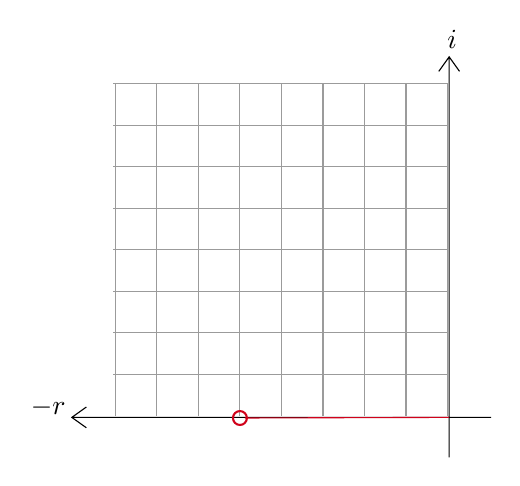
\begin{tikzpicture}[x=0.75pt,y=0.75pt,yscale=-1,xscale=1]
%uncomment if require: \path (0,300); %set diagram left start at 0, and has height of 300

%Shape: Axis 2D [id:dp5907524483347102] 
\draw  (469,209.7) -- (267,209.7)(448.8,36) -- (448.8,229) (274,204.7) -- (267,209.7) -- (274,214.7) (453.8,43) -- (448.8,36) -- (443.8,43)  ;
%Shape: Grid [id:dp6199898397920625] 
\draw  [draw opacity=0] (448,49) -- (287,49) -- (287,209) -- (448,209) -- cycle ; \draw  [color={rgb, 255:red, 155; green, 155; blue, 155 }  ,draw opacity=1 ] (448,49) -- (448,209)(428,49) -- (428,209)(408,49) -- (408,209)(388,49) -- (388,209)(368,49) -- (368,209)(348,49) -- (348,209)(328,49) -- (328,209)(308,49) -- (308,209)(288,49) -- (288,209) ; \draw  [color={rgb, 255:red, 155; green, 155; blue, 155 }  ,draw opacity=1 ] (448,49) -- (287,49)(448,69) -- (287,69)(448,89) -- (287,89)(448,109) -- (287,109)(448,129) -- (287,129)(448,149) -- (287,149)(448,169) -- (287,169)(448,189) -- (287,189) ; \draw  [color={rgb, 255:red, 155; green, 155; blue, 155 }  ,draw opacity=1 ]  ;
%Straight Lines [id:da9323494469903814] 
\draw [color={rgb, 255:red, 208; green, 2; blue, 27 }  ,draw opacity=1 ]   (448.8,209.7) -- (350.35,209.99) ;
\draw [shift={(348,210)}, rotate = 179.83] [color={rgb, 255:red, 208; green, 2; blue, 27 }  ,draw opacity=1 ][line width=0.75]      (0, 0) circle [x radius= 3.35, y radius= 3.35]   ;

% Text Node
\draw (450.23,33) node [anchor=south] [inner sep=0.75pt]    {$i$};
% Text Node
\draw (246,199.4) node [anchor=north west][inner sep=0.75pt]    {$-r$};

\end{tikzpicture}

          \caption{$z=-5$ Plotted on the Imaginary Plane}
          \label{fig:2}
        \end{figure}

      \item $2j$

        $$r=\sqrt{0^2+(2)^2}=2$$
        $$\theta=\frac{\pi}{2}$$
        $$z(r,\theta)=r(\cos(\theta)+j\sin(\theta))$$
        $$z(2,.5\pi)=2j$$
        $$\therefore \text{ In polar: } \boxed{z=2j=2e^{.5\pi j}}$$

        \begin{figure}[H]
          \centering
          \tikzset{every picture/.style={line width=0.75pt}} %set default line width to 0.75pt        

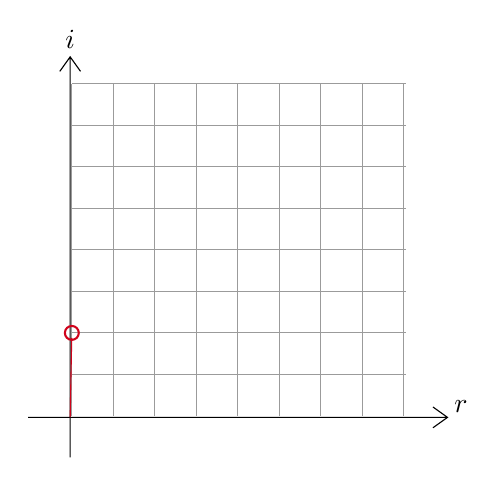
\begin{tikzpicture}[x=0.75pt,y=0.75pt,yscale=-1,xscale=1]
%uncomment if require: \path (0,300); %set diagram left start at 0, and has height of 300

%Shape: Axis 2D [id:dp5907524483347102] 
\draw  (267,209.7) -- (469,209.7)(287.2,36) -- (287.2,229) (462,204.7) -- (469,209.7) -- (462,214.7) (282.2,43) -- (287.2,36) -- (292.2,43)  ;
%Shape: Grid [id:dp6199898397920625] 
\draw  [draw opacity=0] (288,49) -- (449,49) -- (449,209) -- (288,209) -- cycle ; \draw  [color={rgb, 255:red, 155; green, 155; blue, 155 }  ,draw opacity=1 ] (288,49) -- (288,209)(308,49) -- (308,209)(328,49) -- (328,209)(348,49) -- (348,209)(368,49) -- (368,209)(388,49) -- (388,209)(408,49) -- (408,209)(428,49) -- (428,209)(448,49) -- (448,209) ; \draw  [color={rgb, 255:red, 155; green, 155; blue, 155 }  ,draw opacity=1 ] (288,49) -- (449,49)(288,69) -- (449,69)(288,89) -- (449,89)(288,109) -- (449,109)(288,129) -- (449,129)(288,149) -- (449,149)(288,169) -- (449,169)(288,189) -- (449,189) ; \draw  [color={rgb, 255:red, 155; green, 155; blue, 155 }  ,draw opacity=1 ]  ;
%Straight Lines [id:da9323494469903814] 
\draw [color={rgb, 255:red, 208; green, 2; blue, 27 }  ,draw opacity=1 ]   (287.2,209.7) -- (287.95,171.35) ;
\draw [shift={(288,169)}, rotate = 271.13] [color={rgb, 255:red, 208; green, 2; blue, 27 }  ,draw opacity=1 ][line width=0.75]      (0, 0) circle [x radius= 3.35, y radius= 3.35]   ;

% Text Node
\draw (287.23,33) node [anchor=south] [inner sep=0.75pt]    {$i$};
% Text Node
\draw (471,200.4) node [anchor=north west][inner sep=0.75pt]    {$r$};

\end{tikzpicture}

          \caption{$z=2j$ Plotted on the Imaginary Plane}
          \label{fig:3}
        \end{figure}

      \item $\frac{1}{4}(1-j)^5$

        $$.25(1-j)^2(1-j)^3$$
        $$.25(-2j)(1-j)(1-j)^2$$
        $$.25(-2-2j)(-2j)$$
        $$z=j-1$$
        $$r=\sqrt{1^2+(-1)^2}=\sqrt{2}$$
        $$\theta=\frac{3\pi}{4}$$
        $$z(r,\theta)=r(\cos(\theta)+j\sin(\theta))$$
        $$z(\sqrt{2},.75\pi)=j-1$$
        $$\therefore \text{ In polar: } \boxed{z=j-1=\sqrt{2}e^{.75\pi j}}$$

        \begin{figure}[H]
          \centering
          \include{Figures/Fig1d}
          \caption{$z=\frac{1}{4}(1-j)^5$ Plotted on the Imaginary Axis}
          \label{fig:4}
        \end{figure}

      \item $\frac{(1+j)}{j}e^{\frac{j\pi}{3}}$

        $$\frac{(1+j)}{j}\cdot\frac{-j}{-j}=1-j$$
        $$\tan\left( \frac{\pi}{3} \right)=\frac{b}{a}$$
        $$\frac{b}{a}=\sqrt{3}$$
        $$b=a\sqrt{3}$$
        $$\sqrt{(a\sqrt{3})^2+a^2}=1$$
        $$4a^2=\pm1$$
        $$a=\frac{1}{2}$$
        $$b=\frac{\sqrt{3}}{2}$$
        $$\frac{1}{2}(1-j)(1+\sqrt{3}j)\to\frac{1}{2}((\sqrt{3}+1)+(\sqrt{3}-1)j)$$
        $$r=\frac{1}{2}\sqrt{(\sqrt{3}+1)^2+(\sqrt{3}-1)^2}=\sqrt{(4+2\sqrt{3})+(4-2\sqrt{3})}$$
        $$r=\sqrt{2}$$
        $$\theta=\tan^{-1}\left( \frac{\sqrt{3}-1}{\sqrt{3}+1} \right)=.26179$$
        $$z(r,\theta)=r(\cos(\theta)+j\sin(\theta))$$
        $$z(\sqrt{2},.26179)=\frac{1}{2}(\sqrt{3}+1)+(\sqrt{3}-1)j$$
        $$\therefore \text{ In polar: } \boxed{z=\frac{1}{2}(\sqrt{3}+1)+(\sqrt{3}-1)j=\sqrt{2}e^{.26179j}}$$

        \begin{figure}[H]
          \centering
          \include{Figures/Fig1e}
          \caption{$z=\frac{(1+j)}{j}e^{\frac{j\pi}{3}}$ Plotted on the Imaginary Axis}
          \label{fig:5}
        \end{figure}

      \item $(\sqrt{3}-j^5)(1+j)$

        $$j^5=j\to (\sqrt{3}-j)(1+j)=(\sqrt{3}+(\sqrt{3}-1)j+1)$$
        $$(\sqrt{3}+1)+(\sqrt{3}-1)j$$
        $$r=\sqrt{(\sqrt{3}+1)^2+(\sqrt{3}-1)^2}=\sqrt{(4+2\sqrt{3})+(4-2\sqrt{3})}$$
        $$r=\sqrt{8}=2\sqrt{2}$$
        $$\theta=\tan^{-1}\left( \frac{\sqrt{3}-1}{\sqrt{3}+1} \right)=.26179$$
        $$z(r,\theta)=r(\cos(\theta)+j\sin(\theta))$$
        $$z(2\sqrt{2},.26179)=(\sqrt{3}+1)+(\sqrt{3}-1)j$$
        $$\therefore \text{ In polar: } \boxed{z=(\sqrt{3}+1)+(\sqrt{3}-1)j=2\sqrt{2}e^{.26179j}}$$

        \begin{figure}[H]
          \centering
          \include{Figures/Fig1f}
          \caption{$z=(\sqrt{3}-j^5)(1+j)$ Plotted on the Imaginary Axis}
          \label{fig:6}
        \end{figure}

      \item $\frac{2(\sqrt{3}-j)}{1+j\sqrt{3}}$

        $$\frac{2\sqrt{3}-2j}{1+j\sqrt{3}}\cdot\frac{1-j\sqrt{3}}{1-j\sqrt{3}}=-2j$$
        $$r=\sqrt{0^2+(-2)^2}=2$$
        $$\theta=\frac{3\pi}{2}$$
        $$z(r,\theta)=r(\cos(\theta)+j\sin(\theta))$$
        $$z(2,1.5\pi)=-2j$$
        $$\therefore \text{ In polar: } \boxed{z=-2j=2e^{1.5\pi j}}$$

        \begin{figure}[H]
          \centering
          \tikzset{every picture/.style={line width=0.75pt}} %set default line width to 0.75pt        

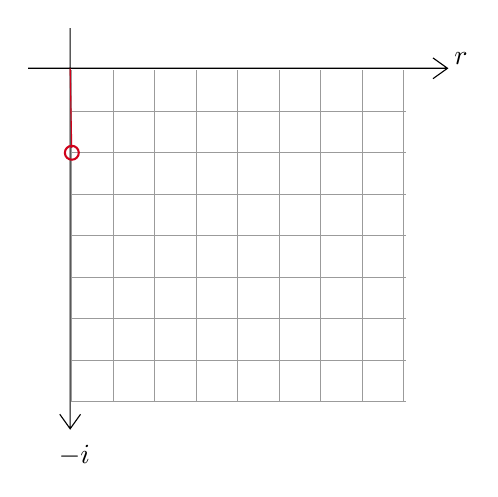
\begin{tikzpicture}[x=0.75pt,y=0.75pt,yscale=-1,xscale=1]
%uncomment if require: \path (0,300); %set diagram left start at 0, and has height of 300

%Shape: Axis 2D [id:dp5907524483347102] 
\draw  (267,55.3) -- (469,55.3)(287.2,229) -- (287.2,36) (462,60.3) -- (469,55.3) -- (462,50.3) (282.2,222) -- (287.2,229) -- (292.2,222)  ;
%Shape: Grid [id:dp6199898397920625] 
\draw  [draw opacity=0] (288,216) -- (449,216) -- (449,56) -- (288,56) -- cycle ; \draw  [color={rgb, 255:red, 155; green, 155; blue, 155 }  ,draw opacity=1 ] (288,216) -- (288,56)(308,216) -- (308,56)(328,216) -- (328,56)(348,216) -- (348,56)(368,216) -- (368,56)(388,216) -- (388,56)(408,216) -- (408,56)(428,216) -- (428,56)(448,216) -- (448,56) ; \draw  [color={rgb, 255:red, 155; green, 155; blue, 155 }  ,draw opacity=1 ] (288,216) -- (449,216)(288,196) -- (449,196)(288,176) -- (449,176)(288,156) -- (449,156)(288,136) -- (449,136)(288,116) -- (449,116)(288,96) -- (449,96)(288,76) -- (449,76) ; \draw  [color={rgb, 255:red, 155; green, 155; blue, 155 }  ,draw opacity=1 ]  ;
%Straight Lines [id:da9323494469903814] 
\draw [color={rgb, 255:red, 208; green, 2; blue, 27 }  ,draw opacity=1 ]   (287.2,55.3) -- (287.95,93.65) ;
\draw [shift={(288,96)}, rotate = 88.87] [color={rgb, 255:red, 208; green, 2; blue, 27 }  ,draw opacity=1 ][line width=0.75]      (0, 0) circle [x radius= 3.35, y radius= 3.35]   ;

% Text Node
\draw (289.23,248) node [anchor=south] [inner sep=0.75pt]    {$-i$};
% Text Node
\draw (471,46.4) node [anchor=north west][inner sep=0.75pt]    {$r$};

\end{tikzpicture}

          \caption{$z=\frac{2(\sqrt{3}-j)}{1+j\sqrt{3}}$ Plotted on the Imaginary Axis}
          \label{fig:7}
        \end{figure}

    \end{enumerate}

  \item Determine the value of $E_{\infty}$ and $P_{\infty}$ for each of the following signals and indicate whether the signal is a power or energy signal or neither.

    \begin{enumerate}

      \item $x_1(t)=\left\{\begin{array}{l r} 5e^{j(4t+\pi/3)},\, & t\geq 2\\ 0,\, & \text{Otherwise}\end{array}$

          $$E_{\infty}=\int_2^{2+\frac{\pi}{4}} 25e^{j(8t+2\pi/3)}\,dt$$
          $$E_{\infty}=\frac{25}{8}\left[ \sin\left( \frac{24t+2\pi}{3} \right)-i\cos\left( \frac{24t+2\pi}{3} \right) \right]\Big|_2^{2+\frac{\pi}{4}}$$
          $$E_{\infty}=2.2755+76.43285i+2.142+2.2755i$$
          $$\therefore\text{ Energy if finite}$$

      \item $x_2(t)=\left\{\begin{array}{l r} 2+2\cos(t),\, & 0<t< 2\pi\\ 0,\, & \text{Otherwise}\end{array}$

          $$P_{\infty}=\lim_{T\to\infty}\frac{1}{2T}\int_{-T}^{T}(2+2\cos(t))^2\,dt$$
          $$P_{\infty}=6$$
          $$\therefore\text{ Power is finite}$$

          $$E_{\infty}=\lim_{T\to\infty}\int_{-T}^T(2+2\cos(t))^2\,dt$$
          $$P_{\infty}=\infty$$
          $$\therefore\text{ Energy is infinite}$$

          \begin{center}
            $$\boxed{\text{Since power is finite and energy is infinite, this is a power signal}}$$
          \end{center}

        \item $x_3[n]=\left\{\begin{array}{l r} (.5)^n,\, & n\geq0\\ 0,\, & \text{Otherwise}\end{array}$

    \end{enumerate}

  \item For the discrete time signal shown in Figure P1.3, sketch, and carefully label each of the following.

    \begin{enumerate}

      \item $x[n-4]$

      \item $x[2n+2]$

    \end{enumerate}

  \item For the continuous time signal shown in Figure P1.4, sketch, and carefully label each of the following.

    \begin{enumerate}

      \item $x(t+3)$

      \item $x\left( 3-\frac{2}{3}t \right)$

    \end{enumerate}

  \item Determine and sketch the even and odd parts of the signals depicted in Figure P1.5. Label your sketches carefully.

    \begin{enumerate}

      \item 

      \item 

    \end{enumerate}

  \item Determine and sketch the even and odd parts of the signal depicted in Figure P1.6. Label your sketches carefully.

  \item Express the real part of each of the following signals in the form $Ae^{-at}\cos(\omega t + \phi)$ where $A$, $a$, $\omega$ and $\phi$ are real numbers with $A > 0$ and $-\pi < \phi \leq \pi$.

    \begin{enumerate}

      \item $x_1(t)=4e^{-2t}\sin\left( 10t+\frac{3\pi}{4}\right)\cos\left( 10t+\frac{3\pi}{4} \right)$

      \item $x_2(t)=j(1-j)e^{(-5+j\pi)t}$

    \end{enumerate}

  \item Determine whether each of the following continuous time signals is periodic. If the signal is periodic, determine its fundamental period.

    \begin{enumerate}

      \item $x(t)=5\cos\left( 400\pi t+\frac{\pi}{4} \right)$

      \item $x(t)=20e^{j(\pi t-2)}$

      \item $x(t)=2\left[ \sin\left( 50\pi t - \frac{\pi}{3} \right) \right]^2$

      \item $x(t)=\left\{\begin{array}{l r} 2\sin(5\pi t),\, & t\geq 0\\ -2\sin(-5\pi t),\, &t<0\end{array}$

    \end{enumerate}

  \item Determine whether each of the following discrete time signals is periodic. If the signal is periodic, determine its fundamental period.

    \begin{enumerate}

      \item $x[n]=2\cos\left( \frac{7}{11}n+\frac{\pi}{2} \right)$

      \item $x[n]=\cos(\pi n)+4\sin\left( \frac{\pi}{4}n^2 \right)$

      \item $x[n]=3\sin\left( \frac{\pi}{3}n \right)+\cos\left( \frac{\pi}{4}n \right)-3\cos\left( \frac{\pi}{6}n+\frac{\pi}{3} \right)$ 

    \end{enumerate}

\end{enumerate}

\end{document}

